\documentclass[b]{beamer}

\usepackage[french]{babel}
\usepackage[utf8]{inputenc}
\usepackage{subcaption}
\usepackage{graphicx}
\usepackage{amsmath,amsfonts,amsthm}

\usetheme{Antibes}
\AtBeginSection[]{
	\begin{frame}
	\vfill
	\centering
	\begin{beamercolorbox}[sep=8pt,center,shadow=true,rounded=true]{title}
		\usebeamerfont{title}\insertsectionhead\par%
	\end{beamercolorbox}
	\vfill
	\end{frame}
}

\title{\texttt{Analyse Discriminate Linéaire}}
\author{HUYLENBROECK Florent, DELFOSSE Charly, JOSSE Thomas}

\begin{document}
	\begin{frame}
		\titlepage
	\end{frame}

	\begin{frame}
		\frametitle{Table des matières}
		\tableofcontents
	\end{frame}
	\section{Introduction}
	\begin{frame}
		\frametitle{Qu'est-ce que l'ADL?}
		Cette technique fait partie des techniques d'analyse discriminante prédictive. Le but et de pouvoir expliquer et prédire l'appartenance d'un individu à un groupe prédéfini à partir de caractéristiques qui ont été mesurées au préalable à l'aide de variables prédictives.
		On peut la comparer à la régression logistique. 
	\end{frame}
	\begin{frame}
		\frametitle{Variables utilisées}
			$X$ contient les $j$ variables prédictives [$X = (X_1,...,X_j)$], $n$ est le nombre d'observations réparties dans $K$ groupe d'effectifs $n_k$, Y est notre variable à prédire qui prend des valeurs dans l'ensemble \{$y_1,...,y_K$\}.
			$\pi_k = P(Y = y_k)$ et est la probabilité que Y soit dans le groupe $k$, $f_k(x)$ est la densité de probabilité de X dans le groupe k.
			De plus nous allons travailler dans le cas gaussien et donc $X \sim \mathcal{N}(\mu_k,\Sigma_k)$ dans chaque groupe $k$, $E_k$ est le groupe d'individus possédant la modalité k dans l'échantillon et $n_k$ est le cardinal de $E_k$
	\end{frame}
	\section{Fonctionnement}
	\subsection{Règle géométrique}
	\begin{frame}
		\frametitle{But Final}
		Cette règle ne prend en compte aucune hypothèse probabiliste. 
		
		Elle consiste à calculer la distance de x (vecteur des variables explicatives sur un individu que l'on veut classer) à chacun des K centres de gravité $g_1,...,g_K$ et affecter x au groupe \underline{le plus proche}.
		
		Et cette distance du nouvel individu au groupe k peut être trouvée via la formule:
		\[
			d^2(x,g_k) = (x - g_k)'\text{\bf W}^{-1}(x - g_k)
		\]¸
		Où {\bf W} est la matrice des variance-covariance intra-groupe.
	\end{frame}
	\begin{frame}
	\frametitle{Développement}
		Pour pouvoir faire cela, nous allons définir notre fonction linéaire discriminante du groupe k pour savoir si x appartient au groupe k* tel que:
		\[
			k^* = arg \underset{k = 1,...,K}{max} d^2(x,g_k)
		\]
		 que l'on peut réécrire:
		\[
		k^* = arg \underset{k = 1,...,K}{max} L_K(x)
		\]
		où 
		\[
		L_K(x) = x'\text{\bf W}^{-1}\text{\bf g}_k - \frac{1}{2}\text{\bf g}'_k\text{\bf W}^{-1}g_k
		\]
		Et $L_K(x)$ est notre fonction linéaire discriminante du groupe k.
		
		Chaque $L_K(x)$ définit une fonction score qui donne une note représentant la probabilité d'appartenance au groupe de la fonction linéaire. X est donc affecté au groupe dont le score est le plus grand.
	\end{frame}
	\subsection{Approche statistique}
	\begin{frame}
	\frametitle{La règle bayesienne}
	Cette règle consiste à produire une estimation de la probabilité après notre affectation.
	Cela veut dire que nous devons réaliser une estimation pour une probabilité conditionnelle:
	\[
	P(Y = y_k | X) = \frac{P(Y = y_k) \times P(X| Y = y_k)}{\sum_{i=1}^{K} P(Y = y_i)\times P(X|Y = y_i)}
	\]
	
	Nous avons $P(Y = y_k)$ qui est la probabilité d'appartenance à la classe $y_k$ et $P(X|Y = y_k)$ qui est la fonction de densité des x par rapport à l'appartenance à la classe $y_k$.
	
	Et cette règle permet d'affecter une nouvelle observation x au groupe k* tel que:
	\[
		k^* = arg \underset{k=1,...,K}{max} P(Y = y_k | X)
	\] 
	\[
		k^*= arg \underset{k=1,...,K}{max} \pi_kf_k(x)
	\]	
	\end{frame}
	\begin{frame}
		\frametitle{Hypothèse d'homoscédasticité}
		L'homoscédasticité est le fait que les variances de chaque groupe soit équivalente (son contraire est l'hétéroscédasticité). Cela veut dire que les données sont réparties de la même manière autour de leur moyenne, ou centre de gravité. 
		
		Pour pouvoir effectuer de l'analyse discriminante linéaire c'est la principale hypothèse que l'on doit appliquer à nos données.
	\end{frame}
	
	\begin{frame}
		\frametitle{Développement}
		L'hypothèse respectée on peut réécrire la règle de Bayes telle que :
		\[
			k^* = arg \underset{k=1,...,K}{max}x!\Sigma^{-1}\mu_k - \frac{1}{2}\mu'_k\Sigma^{-1}\mu_k + \ln(\pi_k)
		\]
		Il nous reste à estimer les  paramètres sur l'échantillon d'apprentissage:
		\begin{itemize}
			\item $\mu_k$ est estimée par $g_k = \frac{1}{n_k}\sum_{i\in E_k}x_i$
			\item la matrice W avec $\Sigma$ commune à tous les groupes devient $\text{\bf W} = \frac{1}{n} \sum_{k=1}\sum_{i\in E_k}(x_i - \text{\bf g}_k)(x_i - \text{\bf g}_k)'$ avec biais ou sans biais :$$\text{\bf W} = \frac{1}{n - K}\sum_{k=1}\sum_{i\in E_k}x_i - \text{\bf g}_k)(x_i - \text{\bf g}_k)'$$
		\end{itemize}
	\end{frame}
	\begin{frame}
		\frametitle{Développement (suite)}
		On obtient ainsi notre règle pour classifier nos individus par l'analyse discriminante linéaire:
		\[
			k^* = arg \underset{k=1,...,K}{max}L_k(x)
		\]
		où
		\[
			L_k(x) = x'\text{\bf W}^{-1}\text{\bf g}_k - \frac{1}{2}\text{\bf g}'_k\text{\bf W}^{-1}\text{\bf g}_k + \ln(\hat{\pi}_k)
		\] est la fonction linéaire discriminante du groupe $k$ et où $\hat{\pi}_k = \frac{n_k}{n}$. Elle fonctionne comme dans la règle géométrique.
		
	\end{frame}
	\section{Exemple}
	\begin{frame}
		Pour réaliser notre exemple, nous avons utiliser la fonction \texttt{discrimin} du package \texttt{ade4} de R qui nous a permis de réaliser l'analyse discriminante de la table de données "\emph{chazeb}" qui est fournie avec ce package ainsi que la table "\emph{skulls}" du même package.
	\end{frame}
	\begin{frame}
		\begin{figure}[h]
			\begin{subfigure}[b]{0.4\textwidth}
				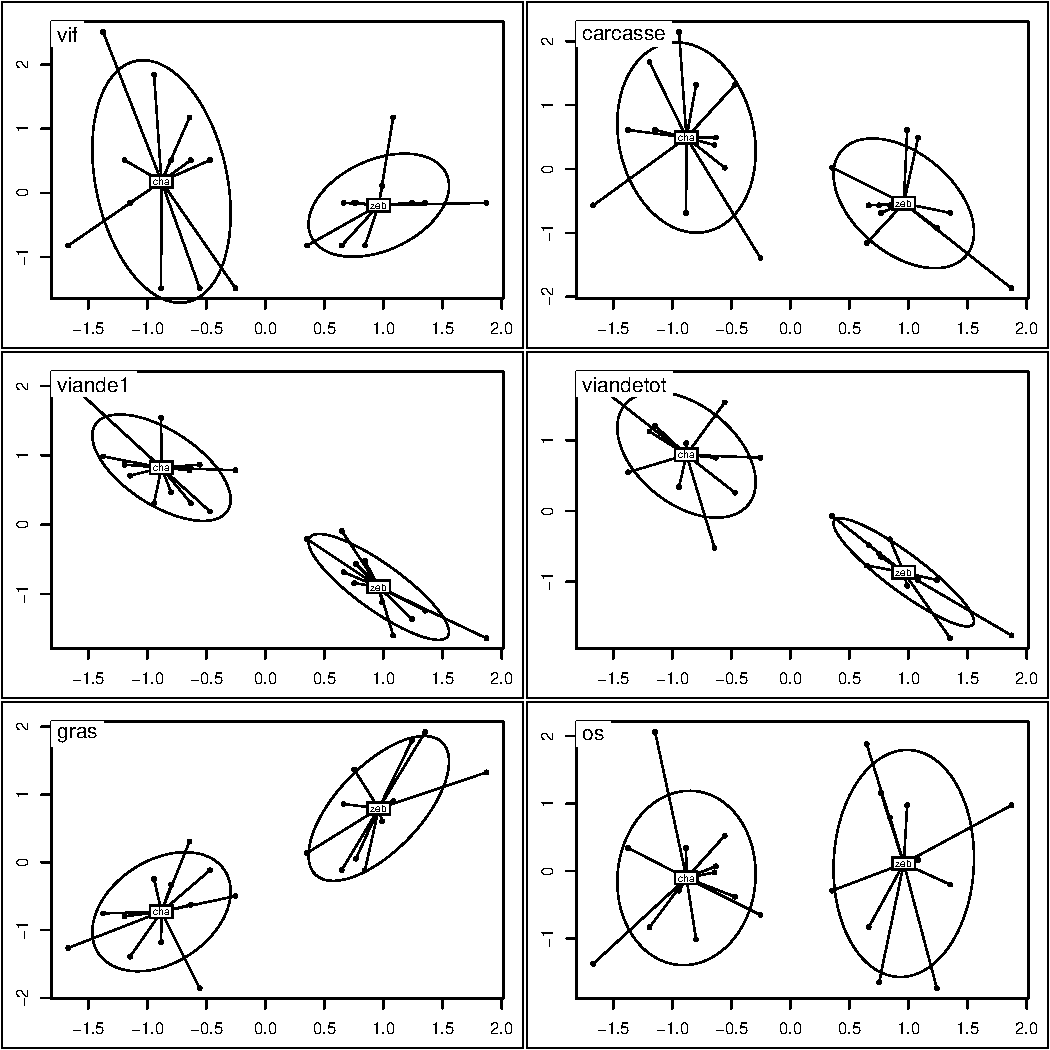
\includegraphics[width=4cm]{Chazeb}
				\caption{Chazeb}
			\end{subfigure}
			\begin{subfigure}[b]{0.4\textwidth}
				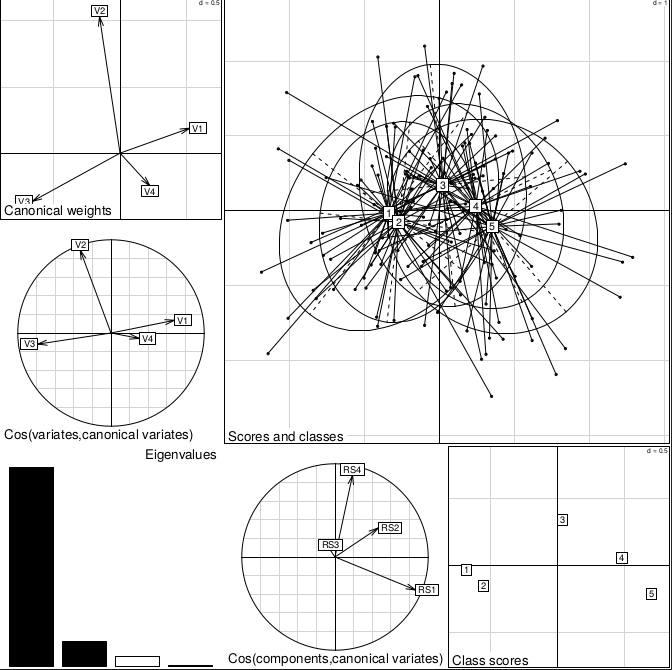
\includegraphics[width=4cm]{Skulls}
				\caption{Skulls}
			\end{subfigure}
		\end{figure}
	\end{frame}
\end{document}